\chapter{Resultados}

\section{Pruebas en los distintos rangos de bits de entrada}

Al emplear el módulo de FixedPointSquareRoot se logra aumentar el dominio de cobertura a la entrada del modulo del RGU, pero dicho módulo aumenta el error al hacer una estimación ya que hace un corrimiento hacia la derecha de los 8 bits menos significativos de la parte entera de los números de entrada en formato de punto fijo.

Entonces sucede que existe una gran variabilidad respecto a los porcentajes de error dependiendo de los rangos mayores a 7 bits, por ejemplo los casos que son de 8 bits en la primera iteración provocan errores de casi el 50 porciento mientras que los casos de 12 bits poseen un error inferior del 1 porciento ante estímulos seudoaleatorios.

\begin{figure}
	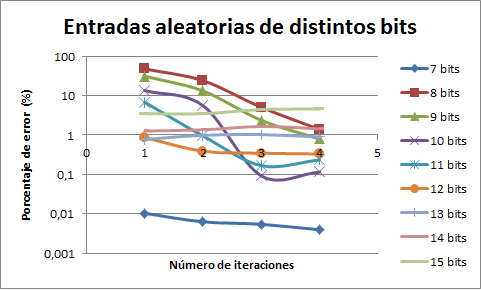
\includegraphics[width=0.7\linewidth]{images/puntos}
	\caption{Gráfico sobre los porcentajes de error ante iteraciones con distintos rangos de bits} \label{fig:puntos}
\end{figure}

En el caso de la figura \ref{fig:puntos} se puede observar que con tres iteraciones el comportamiento de las entradas con 10 bits cambia mucho y para una cuarta iteración más bien sube un poco, lo cual implicaría que más de tres iteraciones en realidad no es necesario para obtener un margen de error apropiado para ese número de iteraciones.

 
%%%%%%%%%%%%%%%%%%%%%%%%%%%%%%%%%%%%%%%%%%%%%%%%%%%%%%%%%%%%%%%%%%%%%%%%%%%%%%%%%%%%%%%%%%%%%%%%%%%%%%%%%%%%
%%%%%%%%%%%%%%%%%%%%%%%%%%%%%%%%%%%%%%%%%%%%%%%%%%%%%%%%%%%%%%%%%%%%%%%%%%%%%%%%%%%%%%%%%%%%%%%%%%%%%%%%%%%%
%%%%%%%%%%%%%%%%%  MACHOTE  %%%%%%%%%%%%%%%%%%%%%%%%%%%%%%%%%%%%%%%%%%%%%%%%%%%%%%%%%%%%%%%%%%%%%%%%%%%%%%%%
%%%%%%%%%%%%%%%%%%%%%%%%%%%%%%%%%%%%%%%%%%%%%%%%%%%%%%%%%%%%%%%%%%%%%%%%%%%%%%%%%%%%%%%%%%%%%%%%%%%%%%%%%%%%
%%%%%%%%%%%%%%%%%%%%%%%%%%%%%%%%%%%%%%%%%%%%%%%%%%%%%%%%%%%%%%%%%%%%%%%%%%%%%%%%%%%%%%%%%%%%%%%%%%%%%%%%%%%%
\begin{comment}


\section{Pruebas para comprobar la funcionalidad y estabilidad}

Al finalizar el desarrollo de la aplicación, se probó acceder a ella desde computadoras en diferentes sistemas operativos. En todos los casos la aplicación operaba de forma correcta. Por lo que independientemente del OS del sistema, la herramienta es funcional, dando como resultado una aplicación web, multiplataforma. Lo cual era uno de los objetivos que se quería alcanzar inicialmente.\\

Además se analizó la exactitud de los datos obtenidos. A la hora de realizar los contornos con la herramienta desarrollado, siempre se obtuvo todos los pixeles que forman parte del mismo, distinto a Sensarea que se obtenían muy pocos puntos si se realizaba la funcionalidad de esta misma manera (dejando precionado el click izquierdo y desplazando el puntero al rededor del contorno).


\section{Pruebas realizadas por diversos usuarios}

Para probar que la aplicación diseñada en efecto es más sencilla de utilizar que las otras herramientas actuales y que con ella se generan datos de manera más eficiente, se procedió a realizar unas pruebas con tiempo a tres diferentes usuarios y se promedió el resultado. Las otras dos herramientas con las cuales se comparó fueron Sensara y VideoANT, debido a que son las únicas que no se requiere de conocimiento técnico para poder instalarlas o utilizarlas en línea. A cada uno se les solicitó realizar las siguientes tareas en orden:

\begin{enumerate}
\item Instalar o acceder a la aplicación
\item Abrir la aplicación, cargar uno de sus video y realizar la segmentación temporal de 5 escenas diferentes.
\item Seguir de la trayectoria de 5 elementos diferentes por al menos 20 cuadros.
\item Dibujar los contornos de 5 elementos diferentes por al menos 20 cuadros.
\item Realizar anotaciones semánticas de 5 tipos diferentes de escenas encontradas.
\end{enumerate}

El video que se utilizó fue una sección de la final de la Copa del Mundo Fifa 2010 entre España y Holanda. El peso del video es de 250 Mb, el formato es mp4 y codec es h264. Los resultados obtenidos se muestran en las tablas \ref{table:results} y \ref{table:results2}. La primera de ellas muestra lo que se duró haciendo la labor por primera vez y en la segunda tabla se muestra el valor promedio de tiempos en las 5 tareas de cada tipo.


\begin{table}[h]\centering
	
	\ra{2}
	\caption{Promedio de tiempo estimado de la primera función realizada correctamente}
	\label{table:results}
	
	\begin{tabular}{@{}cC{3cm}C{3cm}C{3cm}C{3cm}c@{}}\toprule
		
		& Función & GT-Tool & Sensarea & VideoANT&\\ \midrule
		
		& Primer uso de la aplicación & 7 segundos* & 2 minutos & 5 segundos* & \\
		
		& Segmentación temporal  & 26 segundos & 87 segundos & 15 segundos & \\
		
		& Rastreo de objetos & 5 segundos & 5 segundos & no aplica & \\
		
		& Segmentación de contornos & 27 segundos  & 34 segundos & no aplica & \\
		
		& Segmentación semántica & 20 segundos  & no aplica & 15 segundos & \\ 
		
		\bottomrule
		
	\end{tabular}
	
\end{table}

*Ese el tiempo que les tomó acceder a la página web, de lo contrario es el tiempo de descarga e instalación.\\

Se puede apreciar de esta primera tabla (\ref{table:results}), que GT-Tool es muy similar a Sensarea cuando se quiere realizar el seguimiento de la trayectoria de los objetos. Y es un poco más lento que VideoANT a la hora de realizar la segmentación temporal y semántica, esto es debido a la forma en la que VideoANT solicita la información, es más directa pero no tan especializada. De nuevo, VideoANT da precisión de segundos y no de cuadros y además no tiene manera de realizar seguimiento de trayectorias ni segmentación de contornos.\\

A continuación el promedio de las 5 repeticiones luego de haber realizado la tarea por primera vez:


\begin{table}[h]\centering
	
	\ra{2}
	\caption{Promedio de tiempo que tomó realizar cada función repetidas veces (5 repeticiones)}
	\label{table:results2}
	
	\begin{tabular}{@{}cC{3cm}C{3cm}C{3cm}C{3cm}c@{}}\toprule
		
		& Función & GT-Tool & Sensarea & VideoANT&\\ \midrule
		
		& Segmentación temporal  & 19 segundos & 30 segundos & 13 segundos & \\
		
		& Rastreo de objetos & 3 segundos & 4 segundos & no aplica & \\
		
		& Segmentación de contornos & 14 segundos  & 29 segundos & no aplica & \\
		
		& Segmentación semántica & 15 segundos  & no aplica & 13 segundos & \\ 
		
		\bottomrule
		
	\end{tabular}
	
\end{table}

Al analizar los resultados de dicha tabla se concluye los siguiente:

\begin{enumerate}
	
\item A medida que utilizan cualquier herramienta, el tiempo que les toma realizar una labor disminuye, sin importar cual sea. La disminución más grande la tuvo Sensarea en la segmentación temporal, pero esto fue debido a que, aunque Sensarea no soporta nativamente algún tipo de segmentación temporal, se puede simular colocando puntos con etiquetas. Cuando los usuarios se dieron cuenta de esto, lo empezaron a hacer y así hacían un tipo de segmentación temporal.

\item VideoANT continua siendo un poco más rápida para lo temporal y semántico, pero no cuenta con los otros tipos. De igual manera la diferencia en tiempos no es muy significativa.

\item GT-Tool si logra disminuir el tiempo en el que se generan los datos para la trayectoria de objetos y segmentación de contornos, mientras que a la vez aumenta la precisión brindada por Sensarea.

\end{enumerate}

\end{comment}